\chapter{Implementation}
\label{chap:implementation}
\label{sec:implementation}

This chapter describes how the architecture introduced in Chapter~\ref{chap:architecture-requirements} is realised in the ROS~2 workspace. The implementation separates semantic interpretation, planning, deterministic execution, perception grounding, symbolic knowledge, and robot skills. Language-model components interpret requests and propose actions, while typed ROS~2 interfaces and the orchestrator govern execution.

The workspace combines locally developed integration packages with reusable HRI and knowledge components. The implemented contribution is the integration of dialogue management, semantic routing, grounding, planning, orchestration, skills, and feedback into a coherent runtime for the NAO platform.

\section{Runtime Interfaces and Data Contracts}
\label{sec:runtime-contracts}
% ============================================================

The implemented components exchange structured messages so that a language-model output cannot become a robot action without validation. Each contract below identifies the data that crosses one implementation boundary and the component that produces, checks, or consumes it.

\subsection{Runtime Contract Overview}

Table~\ref{tab:contract-map} summarises each runtime contract, its interface or payload, and its owner.

\begin{table}[H]
\centering
\scriptsize
\renewcommand{\arraystretch}{1.18}
\caption{Runtime contract map and ownership in the active dialogue, planning, and execution stack.}
\label{tab:contract-map}

\begin{tabularx}{\textwidth}{
@{}
>{\raggedright\arraybackslash}p{0.04\textwidth}
>{\raggedright\arraybackslash}p{0.17\textwidth}
>{\raggedright\arraybackslash}p{0.38\textwidth}
>{\raggedright\arraybackslash}X
@{}}
\toprule
\textbf{ID} & \textbf{Contract} & \textbf{Interface / payload} & \textbf{Ownership}\\
\midrule

1 & Chatbot turn output
& Internal chatbot result before ROS planner publication.
& \code{dialogue_manager} invokes the chatbot path; \code{chatbot_llm} produces the semantic result.\\

2 & Planner request and admission
& Candidate topic \code{/nao_orchestrator/planner_request}. Admitted topic \code{/planner/request}. Planner-facing payload is carried in \code{Intent.data}.
& \code{chatbot_llm} proposes the execution request; \code{nao_orchestrator} admits and normalizes it; \code{planner_llm} consumes the admitted request.\\

3 & Compact grounding
& \code{grounded_context} inside Contract~2.
& Scene and KB projection provide compact symbolic context for \code{chatbot_llm} and \code{planner_llm}.\\

4 & Shared skill entry
& Registry projection consumed by the planner and orchestrator; its adapter mapping identifies the receiving skill server.
& \code{skill_common} defines the shared capability shape; \code{planner_llm} uses it for prompt construction and \code{nao_orchestrator} uses it for plan validation and dispatch.\\

5 & Planner output
& Topic \code{/intents}. Structured plan payload in \code{Intent.data.plan}.
& \code{planner_llm} produces the plan; \code{nao_orchestrator} validates and dispatches executable steps.\\

6 & Skill execution result
& ROS action result or service response with a typed skill-result payload.
& \code{nao_orchestrator} dispatches the call; the skill server owns fresh evidence; verified world-state updates are applied through \code{kb_skills}.\\

7 & Execution feedback
& Topic \code{/planner/execution_feedback}. Structured JSON feedback payload.
& \code{nao_orchestrator} publishes feedback; a goal-keyed planning-state helper inside \code{planner_llm} uses it for replanning, clarification, or failure handling.\\

8 & Planner dialogue act
& Topic \code{/planner/dialogue_act}. Structured communication request.
& \code{planner_llm} emits dialogue-act intent; \code{nao_orchestrator} relays it; \code{dialogue_manager} realizes the final speech.\\

9 & RDF knowledge state and raw evidence
& KnowledgeCore statements through \code{/kb/query} and \code{/kb/revise}; source evidence includes tracked-person state, \code{/scene/summary}, and skill results.
& Source components own fact freshness; \code{kb_skills} owns KB transport; compact projections and feedback preserve provenance without replacing raw evidence.\\

\bottomrule
\end{tabularx}
\end{table}

The overview keeps only the fields needed to identify each contract. Later sections add the runtime metadata needed for orchestration, feedback-driven planning, tracing, and debugging.

\subsection{Contract 1: Chatbot Turn Output}

The intent in this contract is the user's goal as extracted by the chatbot. It is not a planner output.

\begin{lstlisting}
{
  "verbal_ack": "Okay, I will do that.",
  "route": "execution",
  "confidence": 0.82,
  "user_intent": {
    "type": "look_at",
    "goal_text": "look at the person",
    "scene_targets": ["person"],
    "request_kind": "new_goal"
  }
}
\end{lstlisting}

Table~\ref{tab:chatbot-fields} identifies the fields that remain visible after the chatbot completes one semantic routing decision.

\begin{table}[H]
\centering
\footnotesize
\renewcommand{\arraystretch}{1.18}
\caption{Fields in Contract 1: chatbot turn output.}
\label{tab:chatbot-fields}

\begin{tabularx}{\textwidth}{
@{}
>{\raggedright\arraybackslash}p{0.33\textwidth}
>{\raggedright\arraybackslash}X
@{}}
\toprule
\textbf{Field} & \textbf{Meaning}\\
\midrule

\code{verbal_ack}
& Optional immediate acknowledgement generated by the chatbot layer. This may be spoken or logged before execution begins, depending on the dialogue policy.\\

\code{route}
& Turn classification produced by \code{chatbot_llm}. Supported values include \code{dialogue}, \code{knowledge_query}, and \code{execution}. Only \code{execution} turns enter the planner path; \code{dialogue} and \code{knowledge_query} remain non-execution turns but are still useful for tracing.\\

\code{confidence}
& Confidence assigned by the chatbot or intent-extraction stage. It is useful for debugging and possible admission policy, but it is not a planner priority score.\\

\code{user_intent.type}
& Normalized user-intent label extracted by \code{chatbot_llm}, such as \code{look_at}, \code{find_object}, \code{scan}, or \code{navigate_to}.\\

\code{user_intent.goal_text}
& Natural-language objective passed toward the planner path as the task to satisfy. This field preserves the user's goal in a compact form.\\

\begin{tabular}[t]{@{}l@{}}
\code{user_intent.}\\
\code{scene_targets}
\end{tabular}
& Optional target hints extracted from the utterance, such as \code{person}, \code{cup}, or \code{table}. These are hints, not validated grounded entities.\\

\begin{tabular}[t]{@{}l@{}}
\code{user_intent.}\\
\code{request_kind}
\end{tabular}
& Proposed goal transition class, such as \code{new_goal}, \code{update_goal}, \code{answer_to_clarification}, or \code{cancel_goal}. The planner gate inside \code{nao_orchestrator} should normalize and admit this field before publishing \code{/planner/request}.\\

\bottomrule
\end{tabularx}
\end{table}


\subsection{Contract 2: Planner Request}

The planner request is the task description generated by the orchestrator from the chatbot output and consumed by the planner.

\begin{lstlisting}
{
  "goal_id": "goal_turn_123",
  "request_kind": "new_goal",
  "goal_text": "look at the person and report completion",
  "normalized_intents": ["look_at"],
  "grounded_context": {
    "entities": [
      {
        "id": "anonymous_person_ehfbf",
        "label": null,
        "kind": "person",
        "class": "Human",
        "visible": true,
        "relations": []
      }
    ]
  }
}
\end{lstlisting}

Table~\ref{tab:planner-request-fields} separates request identity, goal semantics, and grounded evidence before the planner is invoked.

\begin{table}[H]
\centering
\footnotesize
\renewcommand{\arraystretch}{1.18}
\caption{Fields in Contract 2: minimal planner-facing request.}
\label{tab:planner-request-fields}

\begin{tabularx}{\textwidth}{
@{}
>{\raggedright\arraybackslash}p{0.33\textwidth}
>{\raggedright\arraybackslash}X
@{}}
\toprule
\textbf{Field} & \textbf{Meaning}\\
\midrule

\code{goal_id}
& Identifier for the active objective. It groups replans and feedback for the same task.\\

\code{request_kind}
& States whether this is a new goal, an update to the current goal, a cancellation, or another supported transition. \code{chatbot_llm} may propose it, but \code{nao_orchestrator} normalizes and admits it before publishing \code{/planner/request}.\\

\code{goal_text}
& Objective extracted from the user utterance. This is the central planning input for \code{planner_llm}.\\

\code{normalized_intents}
& Intent labels extracted by \code{chatbot_llm}. They help \code{planner_llm} choose suitable skills from the available skill registry.\\

\code{grounded_context}
& Compact scene graph used by the planner as the current symbolic state of the world. It contains validated entities and relations rather than raw detector output.\\

\bottomrule
\end{tabularx}
\end{table}

\subsection{Contract 3: Grounded Context}

The planner receives a compact, JSON-native view of relevant world state. This is best described as a compact scene graph derived from the KB, continually updated by the perception pipeline (human/person detection and object perception). Raw KB triples, detector metadata, and tracker-derived details remain available through scene/KB evidence paths to skills, but they are not duplicated into every LLM prompt.

\Needspace{18\baselineskip}
\begin{lstlisting}
{
  "grounded_context": {
    "entities": [
      {
        "id": "cup_jrjic",
        "label": "cup",
        "kind": "object",
        "class": "Cup",
        "visible": true,
        "relations": [
          {"predicate": "dbp:color", "object": "blue"},
          {"predicate": "oro:isOn", "object": "table_1"}
        ]
      },
      {
        "id": "anonymous_person_ehfbf",
        "label": null,
        "kind": "person",
        "class": "Human",
        "visible": true,
        "relations": []
      }
    ]
  }
}
\end{lstlisting}

Table~\ref{tab:grounded-context-fields} defines the compact entity and relation fields used by dialogue and planning.

\begin{table}[H]
\centering
\footnotesize
\renewcommand{\arraystretch}{1.18}
\caption{Fields in Contract 3: grounded context.}
\label{tab:grounded-context-fields}

\begin{tabularx}{\textwidth}{
@{}
>{\raggedright\arraybackslash}p{0.33\textwidth}
>{\raggedright\arraybackslash}X
@{}}
\toprule
\textbf{Field} & \textbf{Meaning}\\
\midrule

\code{id}
& Stable entity handle used by planner steps and skill arguments. This is the preferred reference when a skill needs to target a known person, object, or location.\\

\code{label}
& Human-readable name or class hint. It may be empty for anonymous people or entities that should not be assigned a personal name.\\

\code{kind}
& Entity category, such as \code{object}, \code{person}, or another supported runtime category. This prevents people from being treated as generic objects.\\

\code{class}
& Compact semantic class used by the planner for reasoning, such as \code{Cup}, \code{Human}, or \code{Table}.\\

\code{visible}
& Indicates whether the entity is currently grounded in the latest accepted scene or KB state. It should not be treated as a guarantee that the entity will still be available at execution time.\\

\code{relations}
& Bounded list of relevant semantic relations, such as colour, containment, support, proximity, or ownership-style facts. These relations add task-relevant context without exposing the full KB.\\

\bottomrule
\end{tabularx}
\end{table}

\subsection{Contract 4: Shared Skill Entry}

The planner and orchestrator use one shared entry shape to describe a skill before it is placed in a prompt, admitted for execution, or mapped to an action server. The entry separates the information needed to select a skill from the information needed to verify its result.

\begin{lstlisting}
{
  "object_id": "navigate_to",
  "kind": "skill",
  "category": "navigation",
  "aliases": ["go_to", "move_to_location"],
  "params": ["target", "location"],
  "required_params": ["target"],
  "preconditions": ["navigation is enabled",
                    "target is known or resolvable"],
  "expected_effects": ["robot arrives at the target location"],
  "observable_success": ["status"],
  "failure_modes": ["path_blocked", "unknown_location",
                    "safety_disabled"],
  "planner_guidance": ["use for a semantic destination"],
  "result_schema": {"required": ["skill", "status", "summary_text"]},
  "safety_flags": ["navigation"],
  "implementation_status": "fake",
  "robot_adapter_mapping": "fake_skills.navigate_to",
  "supports_failure_injection": true,
  "metadata": {"runtime_callable": true}
}
\end{lstlisting}

Table~\ref{tab:skill-entry-contract} names the common capability fields consumed by prompt construction, admission, dispatch, and result interpretation.

\begin{table}[H]
\centering
\footnotesize
\renewcommand{\arraystretch}{1.15}
\caption{Shared skill-entry fields used by planning and execution.}
\label{tab:skill-entry-contract}
\begin{tabularx}{\textwidth}{
@{}
>{\raggedright\arraybackslash}p{0.25\textwidth}
>{\raggedright\arraybackslash}X
@{}}
\toprule
\textbf{Field} & \textbf{Runtime role}\\
\midrule
\code{object_id}, \code{kind}, \code{category}, \code{aliases}
& Canonical planner name, semantic group, and accepted compatibility names.\\
\code{params}, \code{required_params}
& Typed planner-facing arguments and the subset required before admission.\\
\code{preconditions}
& Grounding or state assumptions that must be satisfied or explicitly owned by a scenario. They do not prove a future effect.\\
\code{expected_effects}
& Intended state changes or evidence products used to select and order skills.\\
\code{observable_success}
& Result or trace evidence that can support completion after execution.\\
\code{failure_modes}
& Typed outcomes used by the orchestrator and the goal-state helper to stop, clarify, or request replanning.\\
\code{planner_guidance}
& Bounded selection and ordering guidance inserted into the planner prompt.\\
\code{result_schema}
& Required and optional result fields, including the summary and evidence payload.\\
\code{safety_flags}
& Safety-relevant labels used during admission and dispatch.\\
\path{metadata.runtime_callable}
& Whether the registry permits planner-visible runtime use.\\
\code{implementation_status}
& Current implementation class, such as first-party, fake, or hybrid.\\
\code{robot_adapter_mapping}
& Adapter or skill server that receives the dispatched call.\\
\code{supports_failure_}\newline\code{injection}
& Whether controlled failure outcomes are available for validation.\\
\bottomrule
\end{tabularx}
\end{table}

The same shape is projected to the planner prompt, deterministic orchestrator checks, controlled fake skill simulation policies, and adapter configuration. Preconditions constrain admission, while expected effects remain hypotheses until a skill returns observable evidence. This distinction is used by \code{report_result}: a final summary must be derived from result payloads or trace evidence rather than copied from a planner-generated claim. The complete runtime inventory is provided in Appendix~\ref{sec:runtime-skill-inventory}.

\subsection{Contract 5: Planner Output}

The planner output is a plan: a sequence of skill steps to achieve the user goal. It should focus on executable content and minimal lineage. Communication policy and retry metadata are still valid runtime fields when used by the stack, but this controlled version foregrounds the ordered \code{steps} list because that is the essential planner output.

\Needspace{18\baselineskip}
\begin{lstlisting}
{
  "plan": {
    "goal_id": "goal_turn_123",
    "plan_id": "plan_123",
    "plan_version": 1,
    "status": "planned",
    "steps": [
      {
        "id": "step_1",
        "type": "skill",
        "name": "look_at",
        "args": {"target_frame": "anonymous_person_ehfbf"},
        "requires": [],
        "on_failure": "replan"
      }
    ]
  }
}
\end{lstlisting}

Table~\ref{tab:planner-output-fields} identifies the plan and step fields that must survive deterministic validation before dispatch.

\begin{table}[H]
\centering
\footnotesize
\renewcommand{\arraystretch}{1.18}
\caption{Fields in Contract 5: planner output.}
\label{tab:planner-output-fields}

\begin{tabularx}{\textwidth}{
@{}
>{\raggedright\arraybackslash}p{0.32\textwidth}
>{\raggedright\arraybackslash}X
@{}}
\toprule
\textbf{Field} & \textbf{Meaning}\\
\midrule

\code{goal_id}
& User objective that this plan attempts to satisfy. It links the planner output to the active goal.\\

\code{plan_id}
& Identifier for this concrete plan proposal. It is useful when the runtime keeps plan history or compares revised plans for the same goal.\\

\code{plan_version}
& Revision number for replans of the same goal. This helps distinguish the initial plan from later feedback-driven planning outputs.\\

\code{status}
& Planning outcome for this plan, such as \code{planned}, \code{needs_clarification}, or \code{failed_to_plan}. This describes whether \code{planner_llm} produced an executable plan, not whether the robot has already executed it.\\

\code{steps}
& Ordered list of skill calls produced by the planner. This is the essential planner output consumed by \code{nao_orchestrator}.\\

\code{steps[].id}
& Stable step identifier used for execution feedback, dependency tracking, and possible replan joins.\\

\code{steps[].name}
& Skill name selected from the allowed skill registry. The planner should not invent skills or use robot-specific APIs directly.\\

\code{steps[].args}
& Skill arguments. They should refer to known entity IDs, explicit primitive values, or arguments supported by the selected skill schema.\\

\code{steps[].requires}
& Dependencies between steps, if any. This allows the runtime to know which steps depend on previous successful outcomes.\\

\begin{tabular}[t]{@{}l@{}}
\code{steps[].}\\
\code{on_failure}
\end{tabular}
& Recovery policy proposed by \code{planner_llm} for this step. If the step fails, \code{nao_orchestrator} may fail safely, continue if allowed, request user input, or send feedback back to \code{planner_llm} for replanning. Allowed values include \code{replan}, \code{clarify}, \code{ask_user}, \code{continue}, \code{ignore}, and \code{fail}.\\

\bottomrule
\end{tabularx}
\end{table}

\paragraph{Runtime recovery metadata.}
The current contract supports recovery metadata as skill failure may require controlled recovery. Each step may carry a \code{retry_budget}, and the plan envelope may also carry a plan-level \code{retry_budget}. This does not mean that \code{retry} is a separate \code{on_failure} value. Instead, retry behaviour is controlled by \code{nao_orchestrator} using the available retry budget together with the step's \code{on_failure} policy. The plan envelope may also carry \code{communication_policy}. This controls when the planner/dialogue path should communicate progress, completion, clarification needs, or failure.

When a step fails with \code{on_failure = replan}, \code{nao_orchestrator} halts or blocks continuation, publishes execution feedback to \code{planner_llm}, and waits for a revised validated plan before dispatching further actions. This keeps execution authority inside \code{nao_orchestrator}, while allowing recovery to be driven by feedback-driven planning rather than by hard-coded local replanning.

\subsection{Contract 6: Skill Execution Result}

Every dispatched skill returns a typed result before the orchestrator can mark its step as completed. The result distinguishes the execution status from the evidence that supports it. For state-changing skills, the evidence may also describe world-state changes that must be reflected in the KB. These changes are reported by the skill that observed or produced them; they are not inferred from the planner's expected-effects text in Contract~4.

\begin{lstlisting}
{
  "skill": "place_object",
  "status": "succeeded",
  "summary_text": "I placed cup_1 on table_1.",
  "evidence": {
    "object_id": "cup_1",
    "destination_id": "table_1",
    "kb_effects": [
      {"operation": "remove", "statement": "robot oro:holds cup_1"},
      {"operation": "add", "statement": "cup_1 oro:isOn table_1"}
    ]
  },
  "failure": null,
  "metadata": {"fake": true}
}
\end{lstlisting}

The implementation retains the field name \code{evidence.kb_effects}, but the field describes observed world-state changes that must be reflected in the KB and the orchestrator applies these statements only after a successful result.

\subsection{Contract 7: Execution Feedback}

Execution feedback tells the planner which goal and step were affected, whether the step succeeded or failed, and why. This compact information is sufficient to decide whether to continue, replan, request clarification, or report failure.

\Needspace{18\baselineskip}
\begin{lstlisting}
{
  "goal_id": "goal_turn_123",
  "status": "failed",
  "step": {
    "id": "step_1",
    "name": "look_at"
  },
  "reason": "target frame unavailable",
  "result_payload": {
    "target_found": false,
    "target_kind": "person"
  }
}
\end{lstlisting}



Runtime feedback may include additional fields used by \code{nao_orchestrator}, logging, and the goal-state helper. Lineage uses \code{plan_id} and \code{plan_version}; event handling may add \code{event_type}, \code{validation_status}, \code{blocking}, and \path{needs_user_input}; observability may add \code{timestamp_sec}, \code{result_summary}, and retry metadata. These fields support execution control and debugging, while the minimal planner-facing feedback remains the goal, step, status, reason, and result payload.

\subsection{Contract 8: Planner Dialogue Act}

Planner dialogue acts represent planner intent to communicate, not direct speech execution. They are relayed through the orchestrator and realized by the dialogue layer.

\begin{lstlisting}
{
  "goal_id": "goal_turn_123",
  "act": "ask_clarification",
  "await_user_response": true,
  "reason": "multiple visible people",
  "text_hint": "Which person should I look at?",
  "slots_needed": ["target_person"]
}
\end{lstlisting}

Allowed dialogue acts are acknowledgement, progress update, clarification, help request, failure explanation, completion notification, and cancellation notification. The planner does not speak directly; it emits a structured communication request.

\subsection{Contract 9: RDF Knowledge State}

The implementation reuses the open-source KnowledgeCore package rather than introducing a new knowledge-base system \parencite{knowledgecore}. KnowledgeCore represents symbolic world state as an RDF-style graph. Each statement has a subject, predicate, and object. Stable subjects identify people, objects, places, supports, and the robot; predicates express class membership, attributes, visibility, containment, and spatial relations. The same statement shape is used by preloaded fixtures, detector-derived object facts, explicit user-authorised KB mutations, and verified post-skill effects.

\begin{lstlisting}
codex_lab_cup rdf:type Cup
codex_lab_cup dbp:color red
codex_lab_cup oro:isOn codex_lab_table
codex_lab_room oro:contains codex_lab_table
person_alex rdf:type Human
myself sees person_alex
\end{lstlisting}

The principal predicate families are shown in Table~\ref{tab:rdf-kb-predicates}. A class statement such as \code{rdf:type Human} also preserves the semantic distinction between a person and an object even when both can be action targets.

\begin{table}[H]
\centering
\footnotesize
\renewcommand{\arraystretch}{1.15}
\caption{Principal RDF-style predicate families used by the runtime KB.}
\label{tab:rdf-kb-predicates}
\begin{tabularx}{\textwidth}{@{}p{0.24\textwidth}p{0.29\textwidth}X@{}}
\toprule
\textbf{Role} & \textbf{Representative predicates} & \textbf{Runtime meaning}\\
\midrule
Entity class & \code{rdf:type} & Distinguishes people, objects, supports, rooms, and other planner-relevant classes.\\
Attributes & \code{dbp:name}, \code{dbp:color} & Provides stable semantic labels and disambiguating properties.\\
Observation & \code{sees}, visual-centre, score, source, and last-seen predicates & Records who observed an entity and the bounded provenance/freshness of a detector observation.\\
Spatial relations & \code{oro:isOn}, \code{oro:isAt}, \code{oro:isIn}, \code{oro:contains} & Represents support, destination, room membership, and containment used by grounding and skill effects.\\
\bottomrule
\end{tabularx}
\end{table}

KB mutations use add, revise, and remove operations on this shared statement form through \code{/kb/revise}; reads use query patterns through \code{/kb/query}. Transient perception facts carry a finite lifespan, while explicit fixture and verified skill-effect facts follow the lifetime declared by their owner. Reused person-perception components publish person identities and tracked state through their public interfaces \parencite{mohamed2020ros4hri}. Object detections are handled separately by \code{nao_scene_grounding}, which publishes \code{/scene/summary} and detector-derived KB statements.

% ============================================================


\section{ROS Components}

Figure~\ref{fig:full-stack-implementation} locates the principal ROS~2 components and the information exchanged between them. It uses one representation of \code{nao_orchestrator}, whose internal responsibilities include planner-request admission and deterministic plan execution, and focuses on the operational path exercised by the implementation.

\begin{landscape}
\begin{figure}[p]
\centering
\begin{tikzpicture}[
  font=\scriptsize,
  >=Latex,
  component/.style={draw,rounded corners,align=center,text width=3.15cm,minimum height=1.15cm,inner sep=4pt},
  external/.style={component,dashed,fill=gray!8},
  dialogue/.style={component,fill=blue!8},
  planning/.style={component,fill=green!10},
  execution/.style={component,fill=purple!8},
  grounding/.style={component,fill=orange!12},
  flow/.style={-{Latex[length=2.2mm]},line width=0.65pt},
  evidence/.style={-{Latex[length=2.0mm]},line width=0.55pt,dashed}
]

\node[external] (user) at (-9.6,5.0) {User input and robot speech};
\node[dialogue] (dm) at (-5.1,5.0) {\code{dialogue_manager}\\turn state and speech ownership};
\node[dialogue] (chat) at (-0.6,5.0) {\code{chatbot_llm}\\response, route, intent, and goal};

\node[grounding] (perception) at (-7.4,1.1) {Perception components\\objects and tracked people};
\node[grounding] (kb) at (-2.9,1.1) {KnowledgeCore and \code{kb_skills}\\symbolic state and query/revision};
\node[grounding] (context) at (1.6,1.1) {\code{grounded_context}\\bounded entities and relations};

\node[planning] (planner) at (-5.1,-3.0) {\code{planner_llm}\\skill-plan generation and feedback-driven replanning};
\node[execution,text width=3.55cm] (orch) at (0.2,-3.0) {\textbf{\code{nao_orchestrator}}\\request admission, plan validation, and dispatch};
\node[component,fill=gray!8] (skills) at (5.5,-3.0) {Skill servers\\perception, motion, navigation, manipulation, reporting};
\node[external] (platform) at (10.0,-3.0) {NAO or simulated skill adapters};

\draw[flow] (user) -- (dm);
\draw[flow] (dm) -- (chat);
\draw[evidence] (perception) -- (kb);
\draw[evidence] (kb) -- (context);
\draw[evidence] (context) -- (chat);
\draw[evidence] (context) to[out=-110,in=70] (planner.north east);
\draw[flow] (chat.south) to[out=-90,in=90] (orch.north);
\draw[flow] (orch) to[bend right=15] (planner);
\draw[flow] (planner) to[bend right=15] (orch);
\draw[flow] (orch) -- (skills);
\draw[flow] (skills) -- (platform);
\draw[flow] (skills) to[bend left=20] (orch);

\end{tikzpicture}
\caption{Full-stack implementation of the modular interaction architecture. Dialogue interpretation and symbolic grounding provide the planner input; \code{nao_orchestrator} admits the request, validates the returned plan, dispatches skill servers, and forwards execution feedback. Robot-facing and simulated adapters share the same typed skill-result boundary.}
\label{fig:full-stack-implementation}
\end{figure}
\end{landscape}

\subsection{\code{dialogue_manager}}

\code{dialogue_manager} is the ROS~2 lifecycle component responsible for multimodal communication between the robot and its interlocutors. Following the upstream package design\footnote{Package source: \url{https://github.com/ieverythng/dialogue_manager}.}, it preserves chronological conversation histories for active interlocutors and associates incoming \code{hri_msgs/LiveSpeech} streams with the relevant dialogue state. The node invokes the chatbot through \code{DialogueInteraction}, exposes the high-level \code{/skill/chat}, \code{/skill/ask}, and \code{/skill/say} interfaces, and realises final user-facing expressions through the configured Say sub-skill.

This ownership boundary is also a runtime constraint. Planning and execution components publish structured communication requests through the designated dialogue interfaces, while \code{dialogue_manager} retains responsibility for the final utterance and its delivery through the speech backend.

Planner dialogue acts return through the same boundary. \code{planner_llm} publishes structured acknowledgement, clarification, failure, or completion acts on \path{/planner/dialogue_act}; \code{nao_orchestrator} relays the admitted act on \path{/nao_orchestrator/planner_dialogue_act}; and the dialogue layer selects the final wording and speech mechanism. This arrangement provides one user-facing speech authority for each semantic event and makes duplicate acknowledgements or completion reports observable during validation.

\subsection{\code{chatbot_llm}}

\code{chatbot_llm} is a lifecycle-managed semantic-routing node built on the existing chatbot scaffold. Its turn callback receives a \code{DialogueInteraction} request and the conversation history assembled by \code{dialogue_manager}. Before response generation or planner handoff, it queries the KB through \code{kb_skills}, reads the most recent \code{/scene/summary}, and passes both sources through the \code{PlannerHandoff} projection helper. The resulting \code{grounded_context}, defined by Contract~3, contains a bounded set of entities, locations, and task-relevant relations instead of raw detector streams or unrestricted KB rows. This projection informs dialogue and knowledge answers on every user turn and is attached to Contract~2 when the selected route produces a planner request.

The turn engine implements the route field from Contract~1 as follows:
\begin{itemize}
  \item A \code{dialogue} route covers conversational and task-discussion turns and does not publish planner work.
  \item A \code{knowledge_query} route answers from current symbolic evidence without causing a physical action. For example, ``what can you see?'' can use the current grounded context, whereas ``scan and tell me what you see'' requests fresh sensing and is eligible for execution.
  \item An \code{execution} route constructs planner-facing metadata such as goal text, request kind, normalised intent hints, and target KB entities. It publishes a candidate request to \code{/nao_orchestrator/planner_request} without constructing the skill sequence itself.
\end{itemize}

The chatbot prompt defines the component role, the permitted routes, the response requirements, and the structured intent fields. Runtime context adds the dialogue history, available skill summary, and grounded entities. In the evaluated \code{response_first} configuration, the first model call produces the acknowledgement and route decision; the intent stage then extracts goal and target metadata under that route. The \code{intent_first} ablation reverses the stage order and constrains response generation with the previously selected route. Both configurations produce the same Contract~1 output and planner-request format, which allows route consistency to be compared without changing downstream interfaces.

Figure~\ref{fig:chatbot-llm-node} summarises the implemented turn path and the two possible outputs: a response returned to the dialogue manager or an execution request submitted for planner admission.

\begin{figure}[H]
\centering
\resizebox{\textwidth}{!}{%
\begin{tikzpicture}[
  font=\scriptsize,
  >=Latex,
  node distance=0.55cm,
  box/.style={draw,rounded corners,align=center,text width=3.0cm,minimum height=0.9cm,inner sep=4pt},
  dialogue/.style={box,fill=blue!8},
  grounding/.style={box,fill=orange!12},
  process/.style={box,fill=gray!7},
  output/.style={box,fill=purple!7},
  arr/.style={-{Latex[length=2mm]},line width=0.6pt},
  support/.style={-{Latex[length=1.8mm]},line width=0.5pt,dashed}
]
\node[dialogue] (turn) {\code{DialogueInteraction}\\conversation state and user turn};
\node[process,right=of turn] (prompt) {Prompt construction\\role, history, routes, and output schema};
\node[process,right=of prompt] (model) {LLM semantic interpretation\\response and intent stages};
\node[output,right=of model] (result) {Contract~1 turn result\\acknowledgement, route, confidence, goal};
\node[grounding,below=0.75cm of prompt] (context) {Grounded context\\KB, scene, and tracked people};
\node[dialogue,above right=0.70cm and -0.15cm of result] (response) {Response returned to \code{dialogue_manager}};
\node[output,below right=0.70cm and -0.15cm of result] (handoff) {Execution request submitted to \code{nao_orchestrator}};
\draw[arr] (turn) -- (prompt);
\draw[arr] (prompt) -- (model);
\draw[arr] (model) -- (result);
\draw[support] (context) -- (prompt);
\draw[arr] (result) -- (response);
\draw[arr] (result) -- (handoff);
\end{tikzpicture}
}
\caption{Internal \code{chatbot_llm} path. Dialogue history and grounded context condition a structured semantic decision that either returns a user-facing response or submits an execution request for admission.}
\label{fig:chatbot-llm-node}
\end{figure}

\subsection{\code{planner_llm}}

\code{planner_llm} is the high-level planning node and contains a goal-keyed planning-state helper for feedback-driven state transitions. The node subscribes to admitted \code{/planner/request} messages instead of directly consuming chatbot output. Through \code{planner_common}, each request is normalised into the canonical contract with goal metadata nested under \code{plan}. The planner prompt combines the goal text, request kind, normalised intent hints, grounded context, the shared skill-entry projection from Contract~4, permitted step types, and the required JSON output envelope.

The planner prompt is assembled from the admitted request, bounded grounded entities, the skill-registry fields relevant to selection and ordering, the permitted step types, and the planner output contract. It specifies the available skills, required arguments, expected effects, observable completion evidence, and failure modes that may require clarification or replanning. This registry projection links the model's language-level proposal to the typed ROS~2 execution surface.

The model response remains a candidate until the planner engine extracts the JSON object, normalises its schema, validates the required metadata and step fields, and applies one bounded repair retry when configured. Unsupported skill names, malformed arguments, invalid recovery policies, or unparseable output become typed failure or clarification outcomes. Valid plans are published on \code{/intents} for independent orchestrator validation.

Evidence-producing plans receive an additional reporting check. When \code{report_result} follows a sensing, navigation, motion, or manipulation skill, \code{planner_common} requires the reporting step to omit planner-authored result wording. Compatibility normalisation removes fields such as \code{summary_text}, \code{result_summary}, \code{text}, \code{message}, and \code{utterance} before validation. The reporting step is later resolved from the preceding Contract~6 result payload, preventing an expected effect from being presented as an observed result.

The node also subscribes to \code{/planner/execution_feedback}. The embedded planning-state helper associates relevant events with the active goal and invokes the planning path when the orchestrator reports completion, failure, a recoverable condition, or a need for user input. The response may be a revised plan or a structured dialogue act. Robot control remains with the orchestrator, while user-facing communication follows the planner-dialogue relay and dialogue manager.

Figure~\ref{fig:planner-llm-node} shows the planner model call together with its validation, retry, feedback, and publication paths.

\begin{figure}[H]
  \centering
  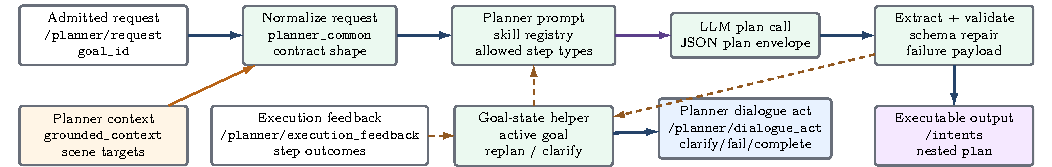
\includegraphics[width=\linewidth]{figures/chapter5_planner_llm.pdf}
  \caption{Internal \code{planner_llm} path, from admitted request through validated plan envelope and feedback-driven goal-state handling.}
  \label{fig:planner-llm-node}
\end{figure}

\subsection{Goal-Keyed Planning-State Helper}

The goal-keyed planning-state helper maintains planning state under an active \code{goal_id}. Each accepted plan carries a \code{plan_id} and monotonically meaningful \code{plan_version}; stable \code{step_id} values allow a newer plan version to preserve completed work when replanning continues the same goal. Feedback from an older or unrelated version is rejected before it can alter the current goal state.

The helper distinguishes planning, replanning, waiting-for-user, completed, and failed states. Step feedback may advance the goal, expose a recoverable condition, or produce a structured dialogue act. If a replacement plan is required, \code{planner_llm} creates and validates it under a newer version. Execution supervision and step dispatch remain within \code{nao_orchestrator}; the helper maintains planning order and lineage across these transitions.

\subsection{Skill Registry (\code{skill_common})}

The planner-facing capability model is derived from the canonical skill registry maintained by \code{skill_common}. Contract~4 and Table~\ref{tab:skill-entry-contract} define the shared entry shape: canonical name and aliases, typed parameters, preconditions, expected effects, observable success evidence, failure modes, result schema, safety flags, runtime availability, and executor mapping. The planner receives a bounded projection of these fields when it selects and orders skills. The orchestrator uses the same names, argument requirements, and availability information when it validates Contract~5 plans and dispatches Contract~6 calls. This arrangement provides a machine-checkable guard against divergence between the prompt-visible capability model and the execution surface.

Table~\ref{tab:runtime-skill-surface} lists the planner-visible skill set. Knowledge-base add, revise, and remove operations remain knowledge-service operations and are not included in this registry. Appendix~\ref{sec:runtime-skill-inventory} gives the arguments, expected evidence, failure modes, and executor for each entry.

\begin{table}[H]
\centering
\scriptsize
\renewcommand{\arraystretch}{1.16}
\caption{Planner-visible skills and their implementations.}
\label{tab:runtime-skill-surface}
\begin{tabularx}{\textwidth}{
@{}
>{\raggedright\arraybackslash}p{0.22\textwidth}
>{\raggedright\arraybackslash}X
>{\raggedright\arraybackslash}p{0.25\textwidth}
>{\raggedright\arraybackslash}p{0.13\textwidth}
@{}}
\toprule
\textbf{Skill} & \textbf{Purpose} & \textbf{Implementation} & \textbf{Controlled simulation}\\
\midrule
\code{scan} & Refresh scene evidence and return a typed scan payload. & First-party \code{/skill/scan} server. & Shared scene-fixture control.\\
\code{find_object} & Find one specified object and return whether it was found. & Perception or simulated adapter. & Yes.\\
\code{inspect_area} & Return the objects and people observed in a specified area. & Perception or simulated adapter. & Yes.\\
\code{navigate_to} & Reach a semantic destination such as a person, object, or location. & Navigation or simulated adapter. & Yes.\\
\code{walk_to} & Execute a short body-relative locomotion segment. & Robot movement or simulated adapter. & Yes.\\
\code{pick_object} & Grasp one specified object and return the observed result. & Manipulation or simulated adapter. & Yes.\\
\code{place_object} & Place a held object at a specified destination. & Manipulation or simulated adapter. & Yes.\\
\code{bring_object} & Deliver one specified object to a person or location. & Composite manipulation or simulated adapter. & Yes.\\
\code{perform_motion} & Execute a named body motion, including a greeting wave. & Motion replay or simulated adapter. & Yes.\\
\code{look_at} & Direct the robot's gaze towards a specified target. & Head, gaze, or simulated adapter. & Yes.\\
\code{ask_user} & Request information needed to continue planning. & Dialogue interface. & Trace-based.\\
\code{report_result} & Report an outcome derived from completed skill results. & Dialogue and reporting interface. & Trace-based.\\
\bottomrule
\end{tabularx}
\end{table}

\subsection{\code{nao_orchestrator} and Plan Execution}

\code{nao_orchestrator} implements deterministic execution of accepted plans. Before dispatch, it validates the plan envelope, ordered steps, registered skill names, arguments, dependencies, failure policies, and goal/plan lineage against the shared skill registry and runtime contracts. A plan is accepted only when every executable step can be resolved to an available skill interface.

Accepted plans are executed in order through the ROS action or skill-server interface mapped by each registry entry. The orchestrator retains the active goal, plan version, current step, completed results, and pending work. For each step it publishes the corresponding started, succeeded, or failed event on \code{/planner/execution_feedback}, preserving the identifiers required to associate execution evidence with the correct goal and plan version.

Each dispatched skill must return a typed Contract~6 result before the step can complete. Successful state-changing results may include world-state updates, which are applied through \code{kb_skills} and verified through a subsequent query when available. On failure, the orchestrator follows the validated step policy: it may stop the plan, continue only when permitted, or publish feedback that requests replanning or clarification. Replacement plans remain the responsibility of \code{planner_llm}.

Figure~\ref{fig:nao-orchestrator-node} summarises the validated plan-execution path described above.

\begin{figure}[H]
\centering
\resizebox{\textwidth}{!}{%
\begin{tikzpicture}[
  font=\scriptsize,
  >=Latex,
  node distance=0.55cm,
  box/.style={draw,rounded corners,align=center,text width=2.9cm,minimum height=0.95cm,inner sep=4pt},
  input/.style={box,fill=green!9},
  execution/.style={box,fill=purple!8},
  result/.style={box,fill=orange!11},
  feedback/.style={box,fill=blue!8},
  arr/.style={-{Latex[length=2mm]},line width=0.6pt},
  support/.style={-{Latex[length=1.8mm]},line width=0.5pt,dashed}
]
\node[input] (plan) {Accepted structured plan\\goal and plan lineage};
\node[execution,right=of plan] (validate) {Plan validation\\skills, arguments, order, and policy};
\node[execution,right=of validate] (dispatch) {Ordered dispatcher\\current step and pending work};
\node[execution,right=of dispatch] (skill) {Skill or adapter call\\typed action/service interface};
\node[result,right=of skill] (result) {Contract~6 result\\status, evidence, world-state updates};
\node[feedback,below=0.8cm of dispatch] (feedback) {Contract~7 feedback\\step and plan events with lineage};
\draw[arr] (plan) -- (validate);
\draw[arr] (validate) -- (dispatch);
\draw[arr] (dispatch) -- (skill);
\draw[arr] (skill) -- (result);
\draw[arr] (result) -- (feedback);
\draw[support] (feedback) -- (dispatch);
\end{tikzpicture}
}
\caption{Execution path implemented by \code{nao_orchestrator}. Accepted plans are validated, dispatched in order, and correlated with typed skill results and execution feedback.}
\label{fig:nao-orchestrator-node}
\end{figure}

\section{World State and Scene Grounding}

The perception path has parallel people and object branches. The person branch reuses \code{hri_face_detect_yunet}, \code{hri_person_manager}, and the ROS4HRI person interfaces to provide identities, tracked-person topics, and frame-qualified state \parencite{mohamed2020ros4hri}. The object branch uses \code{nao_scene_grounding} to convert detector output into a provider-independent scene representation. A custom YOLO detector was trained for a restricted proof-of-concept object set and integrated with the NAO camera stream through ROS. Its strongest demonstration classes are blueberry, corn, pear, tomato, and zucchini. Detector backends are normalised into one internal observation shape so that downstream components do not depend on the detector message type.

The grounding node filters object detections by confidence and an explicit label allowlist, maps labels to KB classes, and maintains local identifiers using tracker IDs or bounded image-plane matching. Without a tracker ID, the default matcher requires the same label, KB class, and detector source, a displacement of at most 64 pixels, and an observation age of at most two seconds. It publishes \code{/scene/summary} and writes accepted observations as transient KnowledgeCore statements through \code{/kb/revise}. Under the default configuration, KB observations have a four-second lifespan and are refreshed no more often than once per second; a local object is removed from the current scene summary after 4.5 seconds without a new detection. An object marked visible in \code{grounded_context} is therefore present in this bounded current-scene window. People remain managed by the tracked-person pipeline and are merged when compact symbolic context is assembled.

\code{kb_skills} provides the query and revision interface for KnowledgeCore. The chatbot formats a bounded query result as an internal knowledge snapshot, combines it with the current scene summary and tracked-person state, and emits the Contract~3 \code{grounded_context}. The projection retains entities, locations, and bounded relations while omitting unrestricted raw rows and detector payloads.

Planning context and execution evidence consequently have different roles. Current symbolic state supports knowledge answers and plan selection. Execution claims require a fresh Contract~6 result from the responsible skill. When \code{pick_object}, \code{place_object}, or \code{bring_object} changes the world state, the result identifies the corresponding removals and additions; the orchestrator reflects them through \code{kb_skills} and verifies the required postconditions when the query interface is available.

Figure~\ref{fig:perception-grounding-pipeline} presents the implemented object, person, knowledge, and compact-grounding paths.

\begin{figure}[H]
\centering
\resizebox{\textwidth}{!}{%
\begin{tikzpicture}[
  font=\scriptsize,
  >=Latex,
  box/.style={draw,rounded corners,align=center,text width=2.9cm,minimum height=0.92cm,inner sep=4pt},
  reused/.style={box,fill=blue!8},
  local/.style={box,fill=orange!11},
  knowledge/.style={box,fill=green!9},
  consumer/.style={box,fill=purple!7},
  arr/.style={-{Latex[length=2mm]},line width=0.6pt},
  support/.style={-{Latex[length=1.8mm]},line width=0.5pt,dashed}
]
\node[local] (camera) at (0,1.5) {NAO camera stream};
\node[local] (detector) at (3.7,1.5) {Object detector\\labels and confidence};
\node[local] (scene) at (7.4,1.5) {\code{nao_scene_grounding}\\normalisation, identity, recency};
\node[local] (summary) at (11.1,1.5) {Object scene state\\\code{/scene/summary}};

\node[reused] (face) at (3.7,-1.2) {ROS4HRI face detector};
\node[reused] (person) at (7.4,-1.2) {\code{hri_person_manager}\\identity and tracked state};
\node[reused] (personstate) at (11.1,-1.2) {Tracked-person interfaces};

\node[knowledge] (kc) at (7.4,-4.0) {KnowledgeCore\\RDF-style world state};
\node[knowledge] (kbskills) at (11.1,-4.0) {\code{kb_skills}\\query and revision interface};
\node[consumer] (context) at (14.8,-1.2) {\code{grounded_context}\\entities and bounded relations};
\node[consumer] (llm) at (18.5,-1.2) {\code{chatbot_llm} and \code{planner_llm}};
\node[consumer] (skills) at (14.8,-4.0) {Execution skills\\fresh scene/KB queries};

\draw[arr] (camera) -- (detector);
\draw[arr] (detector) -- (scene);
\draw[arr] (scene) -- (summary);
\draw[arr] (camera) |- (face);
\draw[arr] (face) -- (person);
\draw[arr] (person) -- (personstate);
\draw[arr] (scene) -- (kc);
\draw[arr] (person) -- (kc);
\draw[arr] (kc) -- (kbskills);
\draw[arr] (summary) -- (context);
\draw[arr] (personstate) -- (context);
\draw[arr] (kbskills) -- (context);
\draw[arr] (context) -- (llm);
\draw[support] (summary) -- (skills);
\draw[support] (kbskills) -- (skills);
\end{tikzpicture}%
}
\caption{Implemented perception and symbolic-grounding pipeline. Reused person-perception components and the local object-grounding path provide bounded scene and knowledge representations to dialogue, planning, and execution skills.}
\label{fig:perception-grounding-pipeline}
\end{figure}

\section{Skill Adapters and Controlled Simulation}

The implementation exposes the planner-visible capabilities in Table~\ref{tab:runtime-skill-surface} through a common adapter boundary. Robot-facing adapters invoke the available physical implementation, whereas the package named \code{fake_skills} supplies deterministic simulated action servers for controlled software evaluation. Both paths preserve the Contract~6 result shape. Simulated results additionally record \code{metadata.fake=true}, the scenario and result mode, the selected policy source, the deterministic seed when applicable, and the simulated duration. Dispatch and outcome events are published on \code{/fake_skills/events}.

The same planner and orchestrator path can therefore be exercised with physical results or with all-success, fail-once, and seeded pseudo-random simulated outcomes. Stateful policies use deterministic call counters and recorded seeds. Successful simulated results represent the corresponding world-state changes, which are reflected in KnowledgeCore so that later plan steps and dialogue turns observe the updated scenario rather than the initial fixture.

Controlled skill-adapter evidence supports software-level claims about route selection, plan validity, ordered dispatch, typed feedback, replanning, clarification, report coverage, and symbolic postconditions. Deterministic simulation also makes it possible to place a known failure at a selected execution step and observe whether the remaining goal is safely replanned. Physical navigation accuracy, grasp reliability, manipulation success, perception accuracy, NAOqi timing, and human-robot safety require separate embodied evaluation.

\section{Models and Runtime Configuration}

The implementation can run with the NAO adapters or deterministic simulated skill adapters while retaining the same dialogue, grounding, planning, orchestration, and result contracts. Model and backend selection are supplied through runtime configuration, so changing an inference provider does not require a different ROS~2 interface.

The primary evaluated configuration uses \code{Qwen3-VL-30B-A3B-Instruct-AWQ} for chatbot and planner inference through an OpenAI-compatible vLLM endpoint. The planner uses temperature \(0.1\) and an 800-token output bound. Additional Qwen3.5 and Ollama-hosted models were exercised over narrower evidence sets and are reported separately in Chapter~\ref{chap:results}.

Interface compatibility does not imply equivalent semantic behaviour. Model, backend, prompt version, sampling configuration, and token limits are therefore recorded as part of the experimental configuration and compared under the controls defined in Chapter~\ref{chap:validation-methodology}.
